% !TeX root = ../main.tex
% Add the above to each chapter to make compiling the PDF easier in some editors.

\chapter{SoTA Quantization Methods}
section investigates how suitable existing SoTA schemes are for comms compression

\section{Numerical experiments}
\begin{itemize}
	\item channel-wise INT, MX, flexgen, topK; explain all of them
    \item table: perplexity increase and bits/value for each method
\end{itemize}

\begin{table}[ht]
\centering
\begin{tabular}{ccccc}
\toprule
 & & \multicolumn{3}{c}{\textbf{Perplexity increase (\%)}}\\

\textbf{Approach} & \textbf{Amort. bits} & \textbf{Gemma-2B} & \textbf{Llama3.1 8B} & \textbf{Mistral 7B} \\
\hline
FP16    & -      & 14.27\%  & 7.22\%  & 5.23\%  \\
\hline
MX4     & 4.25   & 6.18\%   & 3.26\%  & 1.19\%  \\
MX5     & 5.25   & 1.47\%   & 0.75\%  & 0.51\%  \\
MX6     & 6.25   & 0.33\%   & 0.19\%  & 0.17\%  \\
\hline
INT4     & 4.01  & 8.92\%   & 6.08\%  & 17.22\% \\
INT5     & 5.01  & 3.74\%   & 1.63\%  & 7.12\%  \\
INT6     & 6.01  & 1.27\%   & 0.40\%  & 2.04\%  \\
INT8     & 8.01  & 0.08\%   & 0.07\%  & 0.47\%  \\
\hline
Flexgen & 5.00      & 2.71\%   & 1.55\%  & 2.76\%  \\
\bottomrule
\end{tabular}
\caption{Perplexity drop percentages for various approaches, bits per value, and models. 100\% of wikitext test set.}
\end{table}


\subsection{Improving channel-wise INT}
\begin{itemize}
    \item does zero-shifting help?
    \item can we pre-compute zero-shifting values?
\end{itemize}

maybe describe how to determine which approach we should go with... 
e.g. requirement of sub 2\% drop, then pick fastest scheme

\begin{table}[ht]
\centering
\begin{tabular}{ccccccc}
\toprule
 & & & \multicolumn{3}{c}{\textbf{Perplexity increase (\%)}}\\

 \textbf{Bits}& \textbf{Zero-centering} & \textbf{Amort. bits} & \textbf{Gemma-2 2B} & \textbf{Llama3.1 8B} & \textbf{Mistral 7B}  \\
\hline
\multirow{3}{*}{4} & - & 4.01 & 8.2   & 6.4   & 12.8   \\
%4.0 & False & all   & 13.1  & 18.1  & 41.5  & 4.000 \\
 & online & 4.02 & 6.7   & 5.4   & 5.9    \\
%4.0 & True  & all   & 13.4  & 10.2  & 18.0  & 4.000 \\
 & offline & 4.01 & 6.6   & 4.7   & 4.0    \\ \hline
\multirow{3}{*}{5} &  - & 5.01  & 3.6   & 1.6   & 4.9    \\
%5.0 & False & all   & 5.7   & 3.4   & 13.2  & 5.000 \\
 & online & 5.02 & 2.6   & 1.2   & 2.5    \\
%5.0 & True  & all   & 3.8   & 2.6   & 3.9   & 5.000 \\
 & offline & 5.01 & 2.7   & 1.3   & 1.6    \\ \hline
\multirow{3}{*}{6} & - & 6.01  & 1.5   & 0.1   & 1.3    \\
%6.0 & False & all   & 2.3   & 0.2   & 3.8   & 6.000 \\
 & online & 6.02 & 1.1   & 0.6   & 1.1    \\
%6.0 & True  & all   & 1.9   & 0.8   & 0.7   & 6.000 \\
 & offline  & 6.01 & 1.7   & 0.5   & 0.4  \\
\bottomrule
\end{tabular}
\caption{Perplexity increase for different zero-centering approaches. 10\% of wikitext test set.}
\end{table}


\section{(Optimal parametrization of MX schemes)}
paper content
\section{(Random Orthogonal Rotations)}
didn't work, but still put it here? would need additional investigation
\section{Runtime experiments}
\subsection{Method Benchmarking}

\begin{table}[ht]
\centering
\begin{tabular}{ccc}
\toprule
& \multicolumn{2}{c}{\textbf{Runtime (ms)}} \\
\textbf{Approach} & \textbf{Mean} & \textbf{Std} \\ \hline
INT4   & 0.68 & 0.02  \\
INT5   & 0.68 & 0.02 \\
INT6   & 0.69 & 0.02 \\
INT8   & 0.69 & 0.02 \\ \hline
MX4    & 1.84 & 0.06 \\
MX6    & 1.92 & 0.03 \\ \hline
Flexgen & 0.98 & 0.02 \\
\bottomrule
\end{tabular}
\caption{Runtimes for different compiled quantizations schemes.}
\label{tab:runtime_sp} 
\end{table}

\begin{figure}
\centering
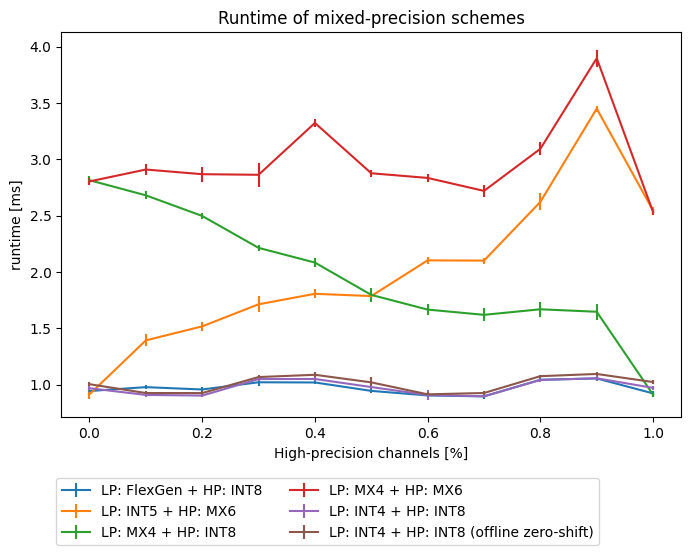
\includegraphics[width=0.8\textwidth]{figures/runtime_mp}
\caption{Outliers within a single layer.}
% Activation shards from the row-wise TP layers are being synchronized using the all\_gather collective op across devices before reduction, which we propose to compress as shown in Figure.}
\label{fig:runtime_mp}
\end{figure}

\begin{itemize}
    \item show column-wise INT is fastest
    \item more fine-grained schemes are much slower
    \item aswell compiled schemes
	\item single-precision Table (\ref{tab:runtime_sp})
	\item mixed-precision Figure (\ref{fig:runtime_mp})
\end{itemize}



\subsection{LLM Benchmarking}
\begin{itemize}
	\item TTFT speedups
	\item takeaway: it's not all about compression rate, but a lot about runtime of approach; INT performs very well but accuracy isn't great
    \item reason for speed difference: for colwise-INT, per-channel scales don't need to be quantized; for block/group quant this is important to keep BPV low
\end{itemize}
takeaway: in the following, we restrict ourselves to experiments dealing only with channel-wise INT quantization, due to their simplicity and good performance


\begin{table}[h]
\centering
\begin{tabular}{llcccc}
\toprule
                &                   &                   & \multicolumn{2}{c}{\textbf{TTFT [s]}}                         &  \\ 
\textbf{Model}  & \textbf{Accelerators} & \textbf{Approach}    & \textbf{Uncompressed} & \textbf{Compressed}    & \textbf{Speedup} \\ 
\midrule
\multirow{4}{*}{LLama 2 70b}  & \multirow{2}{*}{8xL4} & INT4 & 1.07 (0.04) & 0.39 (0.05) & 2.74 \\ 
                            &                                   & MX4 & 1.07 (0.04) & 0.52 (0.63) & 2.06 \\ \cmidrule{2-6}
                            & \multirow{2}{*}{4xA100} & INT4 & 0.13 (0.00) & &\\ 
                            &                                   & MX4 & 0.13 (0.00) & 0.19 (0.00) & 0.68 \\ \midrule
\multirow{2}{*}{Llama 2 13b}  & \multirow{2}{*}{4xL4} & INT4 & 1.37 (0.00) & 0.55 (0.00) & 2.49 \\ 
                            &                                   & MX4 & 1.37 (0.00) & 0.70 (0.00) & 1.96 \\ 
                            \midrule
\multirow{2}{*}{Llama 2 7b}   & \multirow{2}{*}{2xL4} & INT4 & 0.79 (0.00) & 0.66 (0.00) & 1.20 \\ 
                            &                                   & MX4 & 0.79 (0.00) & 0.77 (0.00) & 1.03 \\ 
\bottomrule
\end{tabular}
\caption{Inference profiling results are shown for different models and TP configurations. For compression, quantization scheme with value data type FP4 E2M1, batch size 32 and scale data type E8M0 was used, which has 4.25 effective bits. The TTFT values correspond to the median of 32 model forward passes, additionally we report the standard deviation in brackets. Input shapes 2x128 for 8xL4, 2x256 for 4xA100, 8x256 for 4xL4, 16x256 for 2xL4 were used.}
\label{table:profiling}
\end{table}
